\documentclass[12pt,righttag]{article}

\usepackage{amssymb}
\usepackage{graphicx}

\begin{document}
	\title{The Ising on the Cake}
	\author{Sean Sweany}
	\renewcommand{\today}{April 27, 2016}
	\maketitle
	
	\begin{abstract}
Calculations using the Ising model were done with the Metropolis algorithm to study particle lattices of sizes 2x2, 20x20, 40x40, 60x60 and 80x80 were used in order to find just how the size of the matrix affects the point at where the phase transition takes place. The 2x2 system was explicitly solved for by hand and then compared to the simulations. The 20x20 system was used to study the number of Monte Carlo cycles needed for the solution to converge for both random and aligned particle spin initial configurations, as well as for two different temperatures T=1 and T=2.4. Finally, a temperature gradient of 0.02 was used over a range of T=2 to T=3 to see the phase transition in the above mentioned lattices. Results show that there is clearly a phase transition around Onsanger's value of the critical temperature which is 2.26.
	\end{abstract}

	
	\section{Introduction}
   The Ising model was a problem proposed in the 1920's by Wilhelm Lenz to his student Ernst Ising as something to work on for his thesis work. Ernst was able to solve the Ising model in one dimension, however he never solved it in two[3]. The two dimensional model is interesting because it is able to model phase transitions in ferromagnetic materials where it is assumed there is a lattice of particles with spins oriented either up and down. This phase transition takes place when the spins go from an ordered orientation to one of disorder, which is related to the temperature of the system. In this project we investigate solutions to the Ising model in 2 dimensions for increasing sizes of particle lattices, where it will be shown that at a certain temperature there is indeed a phase transition which takes place[5].


\section{Theory}
\subsection{Thermodynamics of the System}
The Ising model is a statistical physics model used to understand systems of particles, in this model a particle lattice is created where the particles have spins that are either up or down. Without a magnetic field present the energy of this system is described as follows.
\[E=-J\sum_{<ij>}^{N}S_iS_j\] 
where the S's are either +1 or -1, describing the corresponding up and down spins. In the model the summing takes place for a center particle and the four surrounding it, meaning that the energy of contribution from each site is directly related to the four spins closest to it. The model being used makes use of what's known as periodic boundary conditions for calculating the energy. Implementing these boundary conditions for a particle on the edge of the lattice at point $(i,i)$ will use the points $(i-1,i),(i,i-1),(i,0),(0,i)$ for calculating the energy at that lattice point. What's being done here is that when you are at the edge of the lattice for the directions of the 4 particles that go off the lattice you instead use the values of the spins on the opposite side of the lattice. For the system the magnetization of a configuration is just the sum of all S's over the entire lattice. Once both of these are known we can then find the relevant thermodynamical quantities. To do this though we need to find the partition function Z[2].
\[Z=\sum_{i}^{N}e^{-\beta E_i}\]
where $\beta=1/kT$
With this function finding the average energy, magnetization, specific heat  and susceptibility are very simple using the following equations.
\[<E>=\frac{\sum_{i}^{N}E_ie^{-\beta E_i}}{Z}\]
\[<|M|>=\frac{\sum_{i}^{N}|M|_ie^{-\beta E_i}}{Z}\]
\[<H>=\frac{<E^2>-<E>^2}{kT^2}\]
\[<\chi>=\frac{<M^2>-<|M|>^2}{kT}\]

\subsection{Phase Transitions}
A useful behavior that the Ising model exhibits is that for the model in two dimensions and above it is able to predict phase transitions. A phase transition is when the change in external parameters of a system cause a change in the macroscopic properties in the system. These transitions are governed by the correlation length, which is the distance over which degrees of freedom are correlated between the particles. Phase transitions are generally split into two categories, first and second order transitions. In first order transitions the correlation length is a finite value at the critical temperature and the thermodynamic functions for quantities such as energy and entropy exhibit a discontinuity when changing an external variable of the system. For these transitions the two states can coexist for a time until enough energy has been either input or removed from the system for the total transition to occur. The most common example of this is when ice melts and becomes water. In second order transitions the correlation length actually goes to infinity, this makes the entire system suddenly switch to a new state once this temperature is reached. The Ising model in 2d exhibits a second order phase transition with the spontaneous magnetization of all the particles in the lattice[1][2].

An important aspect of the correlation length is that close to the critical temperature it should be on the order of the lattice spacing. Knowing this gives the relation $\eta ~|T_c-T|^{-\nu}$, this equation captures the behavior as T approaches $T_c$ the correlation length diverges to infinity. At the critical point the correlation length will be proportional to the size of the lattice times some constant. What this gives is, where $\nu$ is simply 1[1][2].
\[T_c(L)-T_c(\infty)=aL^{\frac{-1}{\nu}}\]


 

\subsection{Markov Chains}
A Markov chain is defined as given a set of states $S=(s_1,s_2,......s_n)$, starting in a state $s_i$ you move to state $s_j$ with a transition probability $W_{ij}$. This move to a new state is called a step, and taking multiple steps creates a Markov chain. This $W_{ij}$ can be represented as a matrix called the transition matrix. Where the columns of this matrix represent the current state of the system and the rows provide the probability of moving from the current state to a new one. Due to probability conservation this restricts the sum of each column to be 1. Now, looking at this mathematically say we have a probability distribution $w_i(t)$, this can then be represented as follows
\[w_i(t_n)=\sum_{j}W_{ij}(t_n)w_j(0)\]
or, probably a more useful way of writing it is in matrix form
\[\hat{w}(n\epsilon)=\hat{W}^n(\epsilon)\hat{w}(0)\]
This is now an eigenvalue problem, and what will be found is that the largest eigenvalue will be one, and this will then be the steady state solution. The problem with this though is that even though it gives a nice way to understand how a system comes to equilibrium after a certain amount of time we don't really know what anything is. We have no foreseeable way of finding this matrix of transition probabilities. Luckily this problem is solved by use of the Metropolis Algorithm[2].

\subsection{The Roots of the Metropolis Algorithm}
Take the transition probability matrix from above and split it into two different probabilities $W_{ij}=T_{ij}A_{ij}$. Where $T_{ij}$ is the probability of moving to a state j from a state i and $A_{ij}$ is the probability of accepting the move. This means that $1-A_{ij}$ is the probability of not accepting the move. Using this it is easy to rewrite the equation for the probability distribution at a time t as
\[w_i(t+1)=\sum_{j}T_{ji}A_{ji}w_j(t)+w_i(t)T_{ij}(1-A_{ij})\]
But $\sum_{j}T_{ij}=1$ by probability conservation so the equation becomes
\[w_i(t+1)-w_i(t)=\sum_{j}T_{ji}A_{ji}w_j(t)-w_i(t)T_{ij}A_{ij}\]
As time goes to infinity $w_i(t +1)=w_i(t)$, this leads to
\[\sum_{j}T_{ji}A_{ji}w_j(t)=\sum_{j}w_i(t)T_{ij}A_{ij}=w_i\]
Enforcing detailed balance so as to not have cyclic solutions the final solution is just
\[T_{ji}A_{ji}w_j(t)=w_i(t)T_{ij}A_{ij}\]
This leads to the final solution 
\[\frac{T_{ji}A_{ji}}{T_{ij}A_{ij}}=\frac{w_i}{w_j}\]
This equation is now in a form that is useful, because the probability distributions are known and A and T can be found. This is the basis for the Metropolis Algorithm[2].




\section{Numerical Methods}
\subsection{Metropolis Algorithm}
Above the main equation for the Metropolis algorithm was derived, here we will go over how to apply it to the Ising model. First, we need to have a probability distribution, for our case it is the Boltzmann Distribution
\[w_i=\frac{e^{-\beta E_i}}{Z}\]
Taking the fraction of the probability distribution of states i and j the partition function falls out of the equation. Also, if the assumption is made that $T_{ij}=T_{ji}$ the above equation reduces down to 
\[\frac{A_{ji}}{A_{ij}}=e^{-\beta (E_i - E_j)}\]
This is just wonderful because now it is possible find criteria for the acceptance probabilities. The first case is if $\delta E$ is less than or equal to zero. If so $e^{-\beta \delta E}$ is greater than 1, this implies that $\frac{A_{ji}}{A_{ij}}$ is greater than or equal to 1. Now, the largest value of $A_{ji}$ is 1, so for this case just call it that. For the case where $\delta E$ is greater than 0 the situation is reversed giving us that $\frac{A_{ji}}{A_{ij}}$ is less than 1. For this case we then say that $A_{ji}=e^{-\beta \delta E}$. What this gives us then is the situation where if a spin is flipped and the energy is lowered then the new configuration is accepted, but if the energy increases then there is some probability $e^{-\beta \delta E}$ of the move being accepted. The Metropolis algorithm then boils down to this simple recipe.
\begin {enumerate}
\item	Initialize the lattice and calculate the energy 
\item Randomly flip a spin in the lattice 
\item Calculate the energy difference, if the energy difference is negative accept the flip. 
\item If not then generate a random number, if that number is less than $e^{-\beta \delta E}$ accept the flip, if not keep the current configuration. 
\item Repeat this process until equilibrium is reached[2]
\end {enumerate}


The above algorithm is very simple, however it can be time consuming if not implemented in an intelligent way. One thing that can be done to cut down on cpu time is to precalculate the energy differences. In the program, if at each step you calculate the energy difference from the Ising model energy equation this will take a long time. Luckily there are a limited number of configurations so the change in the energy of the system can be precalculated for every step. This value ends up being simply $\delta E=2Js_l^1\sum{k}{N}s_k$, where $s_l^1$ is the value of the spin before flipping. The magnetization can similarly be calculated since flipping a spin will add or subtract 2 from the total magnetization the equation is simply[2] $M_2=M_1+2s_l^2$




\section{Results}
\subsection{2x2 Lattice}
		The average energy, magnetization, specific heat and susceptibility were solved by hand for the 2x2 lattice of particles. This system is nice since it can  be easily calculated by hand using the four equations in the above theory section. Table 1 shows all of the possible energy, magnetizations and degeneracy for all possible spin configurations for the 2x2 system. Knowing these it is then easy to calculate the relevant thermodynamic quantities. The steps are as follows, first find what that partition function for the system is. For this case it is $2(6+e^{8J\beta}+e^{-8J\beta})$. Once this is obtained use the above equations and solve. I will go through the example of finding the energy and provide the solutions to the other three since all this is now is an exercise in algebra.
		\[<E>=\frac{\sum_{i}^{N}E_ie^{-\beta E_i}}{2(6+e^{8J\beta}+e^{-8J\beta})}=\frac{2(-8Je^{8J\beta}+8Je^{-8J\beta})}{2(6+e^{8J\beta}+e^{-8J\beta})}\]
		\[=-8J\frac{\sinh(8J\beta)}{3+\cosh(8J\beta)}\]
		
		\[<|M|>=\frac{2e^{8J\beta}+4}{3+\cosh(8J\beta)}\]
		\[<C>=\frac{64J}{T^2}\frac{3\cosh(8J\beta)+1}{(\cosh(8J\beta)+3)^2}\]
		\[<\chi>=4\frac{3+3e^{8J\beta}+e^{-8J\beta}}{(3+\cosh(8J\beta))^2}\]
		
		
		
	
	\begin{table}
		\begin{center}
			\caption{Variables in the 2x2 System}
			\begin{tabular}{c c c c}
				\hline\hline
				Spins Up & Degeneracy & Energy & Magnetization  \\ 
				\hline
				4 & 1 & -8J & 4\\
				3 & 4 & 0 & 2 \\
				2 & 4 & 0 & 0 \\
				2 & 2 & 8J & 0 \\
				1 & 4 & 0 & -2\\
				0 & 1 & -8J & -4 \\
				
				\hline
			\end{tabular}
		\end{center}
	\end{table}


\begin{table}
	\begin{center}
		\caption{2x2 Thermodynamic Quantities}
		\begin{tabular}{c c c c}
			\hline\hline
			Quantity & Exact & Monte Carlo & Percent Difference  \\ 
			\hline
			Energy & -7.9839 & -7.9845 & 0.0075\\
		    Magnetization & 3.9946 & 3.995 & 0.01 \\
			Specific Heat & 0.1283 & 0.1233 & 3.89 \\
			Susceptibility & 0.01604 & 0.01661 & 3.55 \\
			
			
			\hline
		\end{tabular}
	\end{center}
\end{table}
	
	The above calculations used 1,000,000 Monte Carlo Cycles which was complete overkill, however it did produce very good agreement between the exact solutions and what was calculated. Also, for the 2x2 case, using 1,000,000 Monte Carlo Cycles only takes a few seconds so it is not a very big deal. It should be noted that this was also done for fewer Monte Carlo Cycles, however, in all of those cases both the Specific Heat and Susceptibility were way off from what they were supposed to be. This part sets a benchmark for checking the code as we go further on with the project since we have the exact answer.
	
	\subsection{20x20 Lattice}
	The next thing to be studied was how quickly equilibrium was reached in the 20x20 particle lattice for temperatures of 1 and 2.4 in dimensionless units and for starting particle configurations, where configuration 1 is all spins pointed in the same direction and configuration 2 is where the spins are randomly distributed being either up or down. For this part the average magnetization and average energy were studied. Fig.~\ref{Energy} shows how the average energy is affected by the number or Monte Carlo cycles and different starting configurations and Fig.~\ref{Magnetization} shows the same thing except for the average magnetization. Looking at the figures both the energy and magnetization show very similar behavior to one another. For T=1, when the particles all start off aligned in the same direction the number of Monte Carlo cycles needed to reach equilibrium are very few, taking less then 1000 cycles to converge. If the starting configuration is random then it takes about twice as long to reach equilibrium, however once equilibrium is reached there are jumps where there are sharp spikes in the energy and magnetization only to go back to the equilibrium position at the next Monte Carlo cycle step. For the case where the temperature is 2.4 the results are rather different. For both energy and magnetization the behavior is nearly the same, however now it takes both at least 5000 cycles to come to equilibrium. The interesting thing is that there is much more spread in the values of the energy and magnetization around the average value. This shows that for low temperatures there is very little variance in the value of the average thermodynamic quantities around the mean. After you go past the critical point though the variance around the mean greatly increases.
	
		\begin{figure}
			
			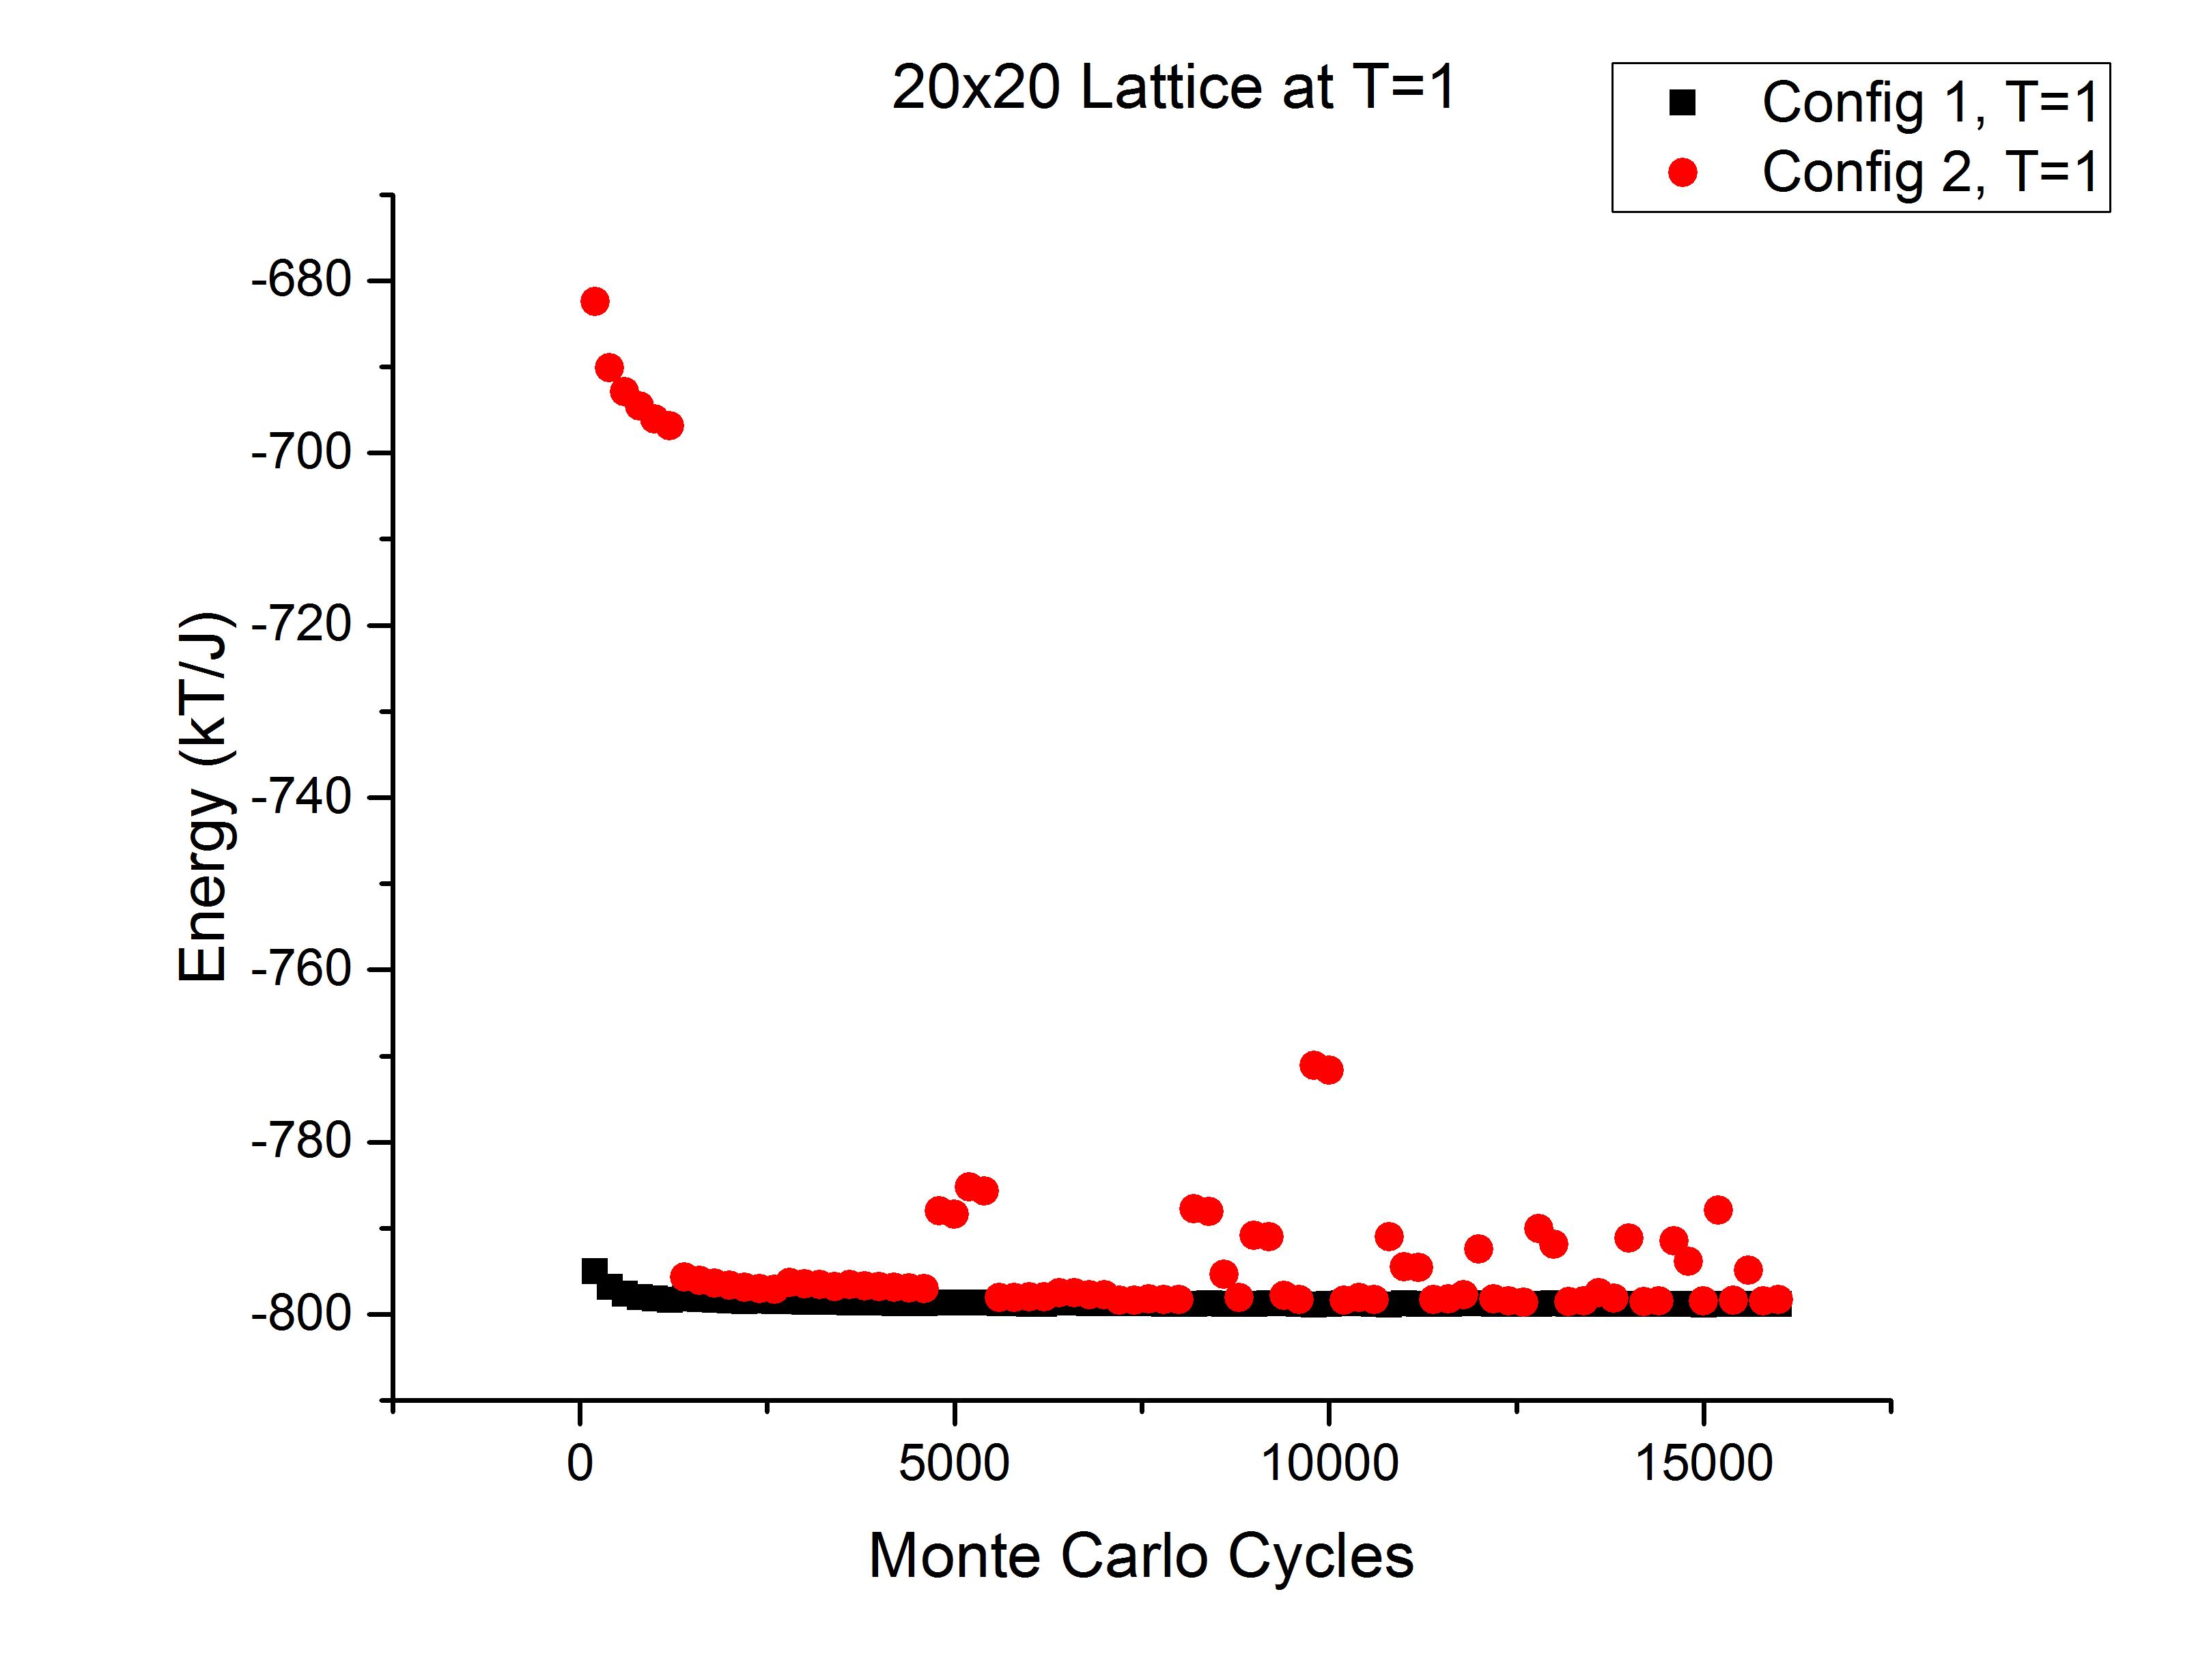
\includegraphics[width=3in]{Graph01.png}
			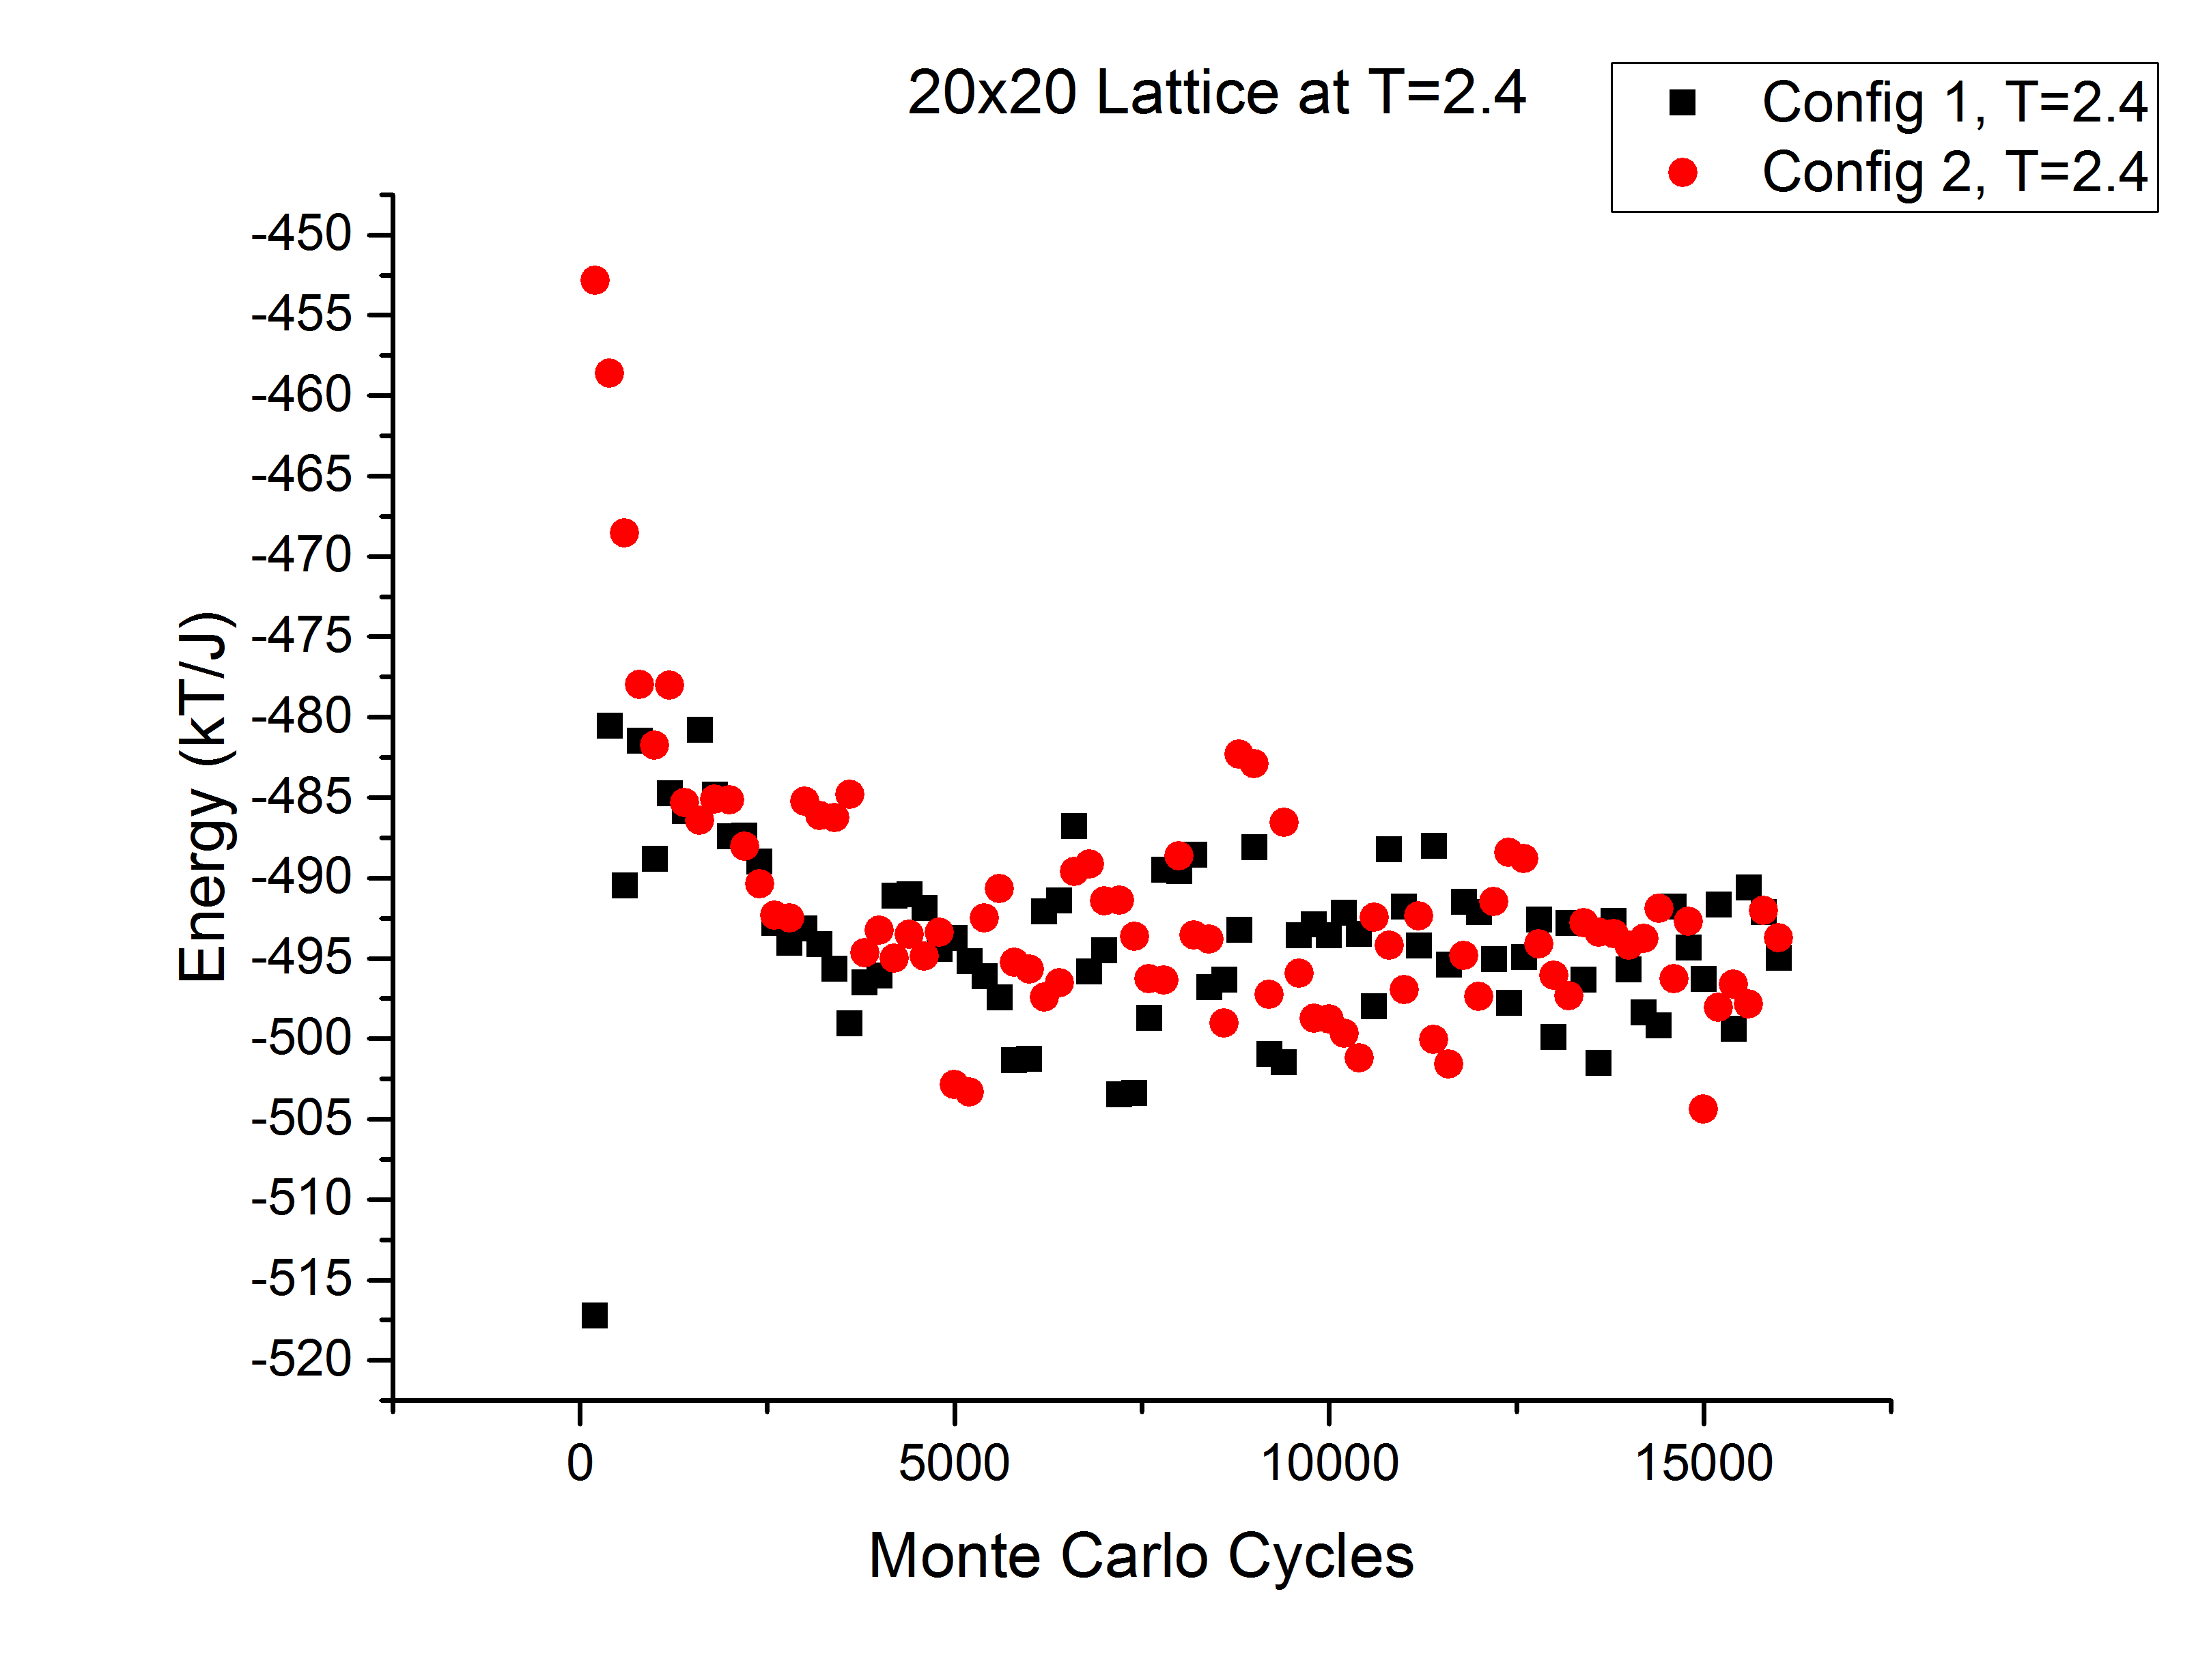
\includegraphics[width=3in]{Graph02.png}
			
			
			\caption{\label{Energy} Average energy for different temperatures and initial configurations (Left) T=1 (Right) T=2.4}
		\end{figure}
		
		\begin{figure}
			
			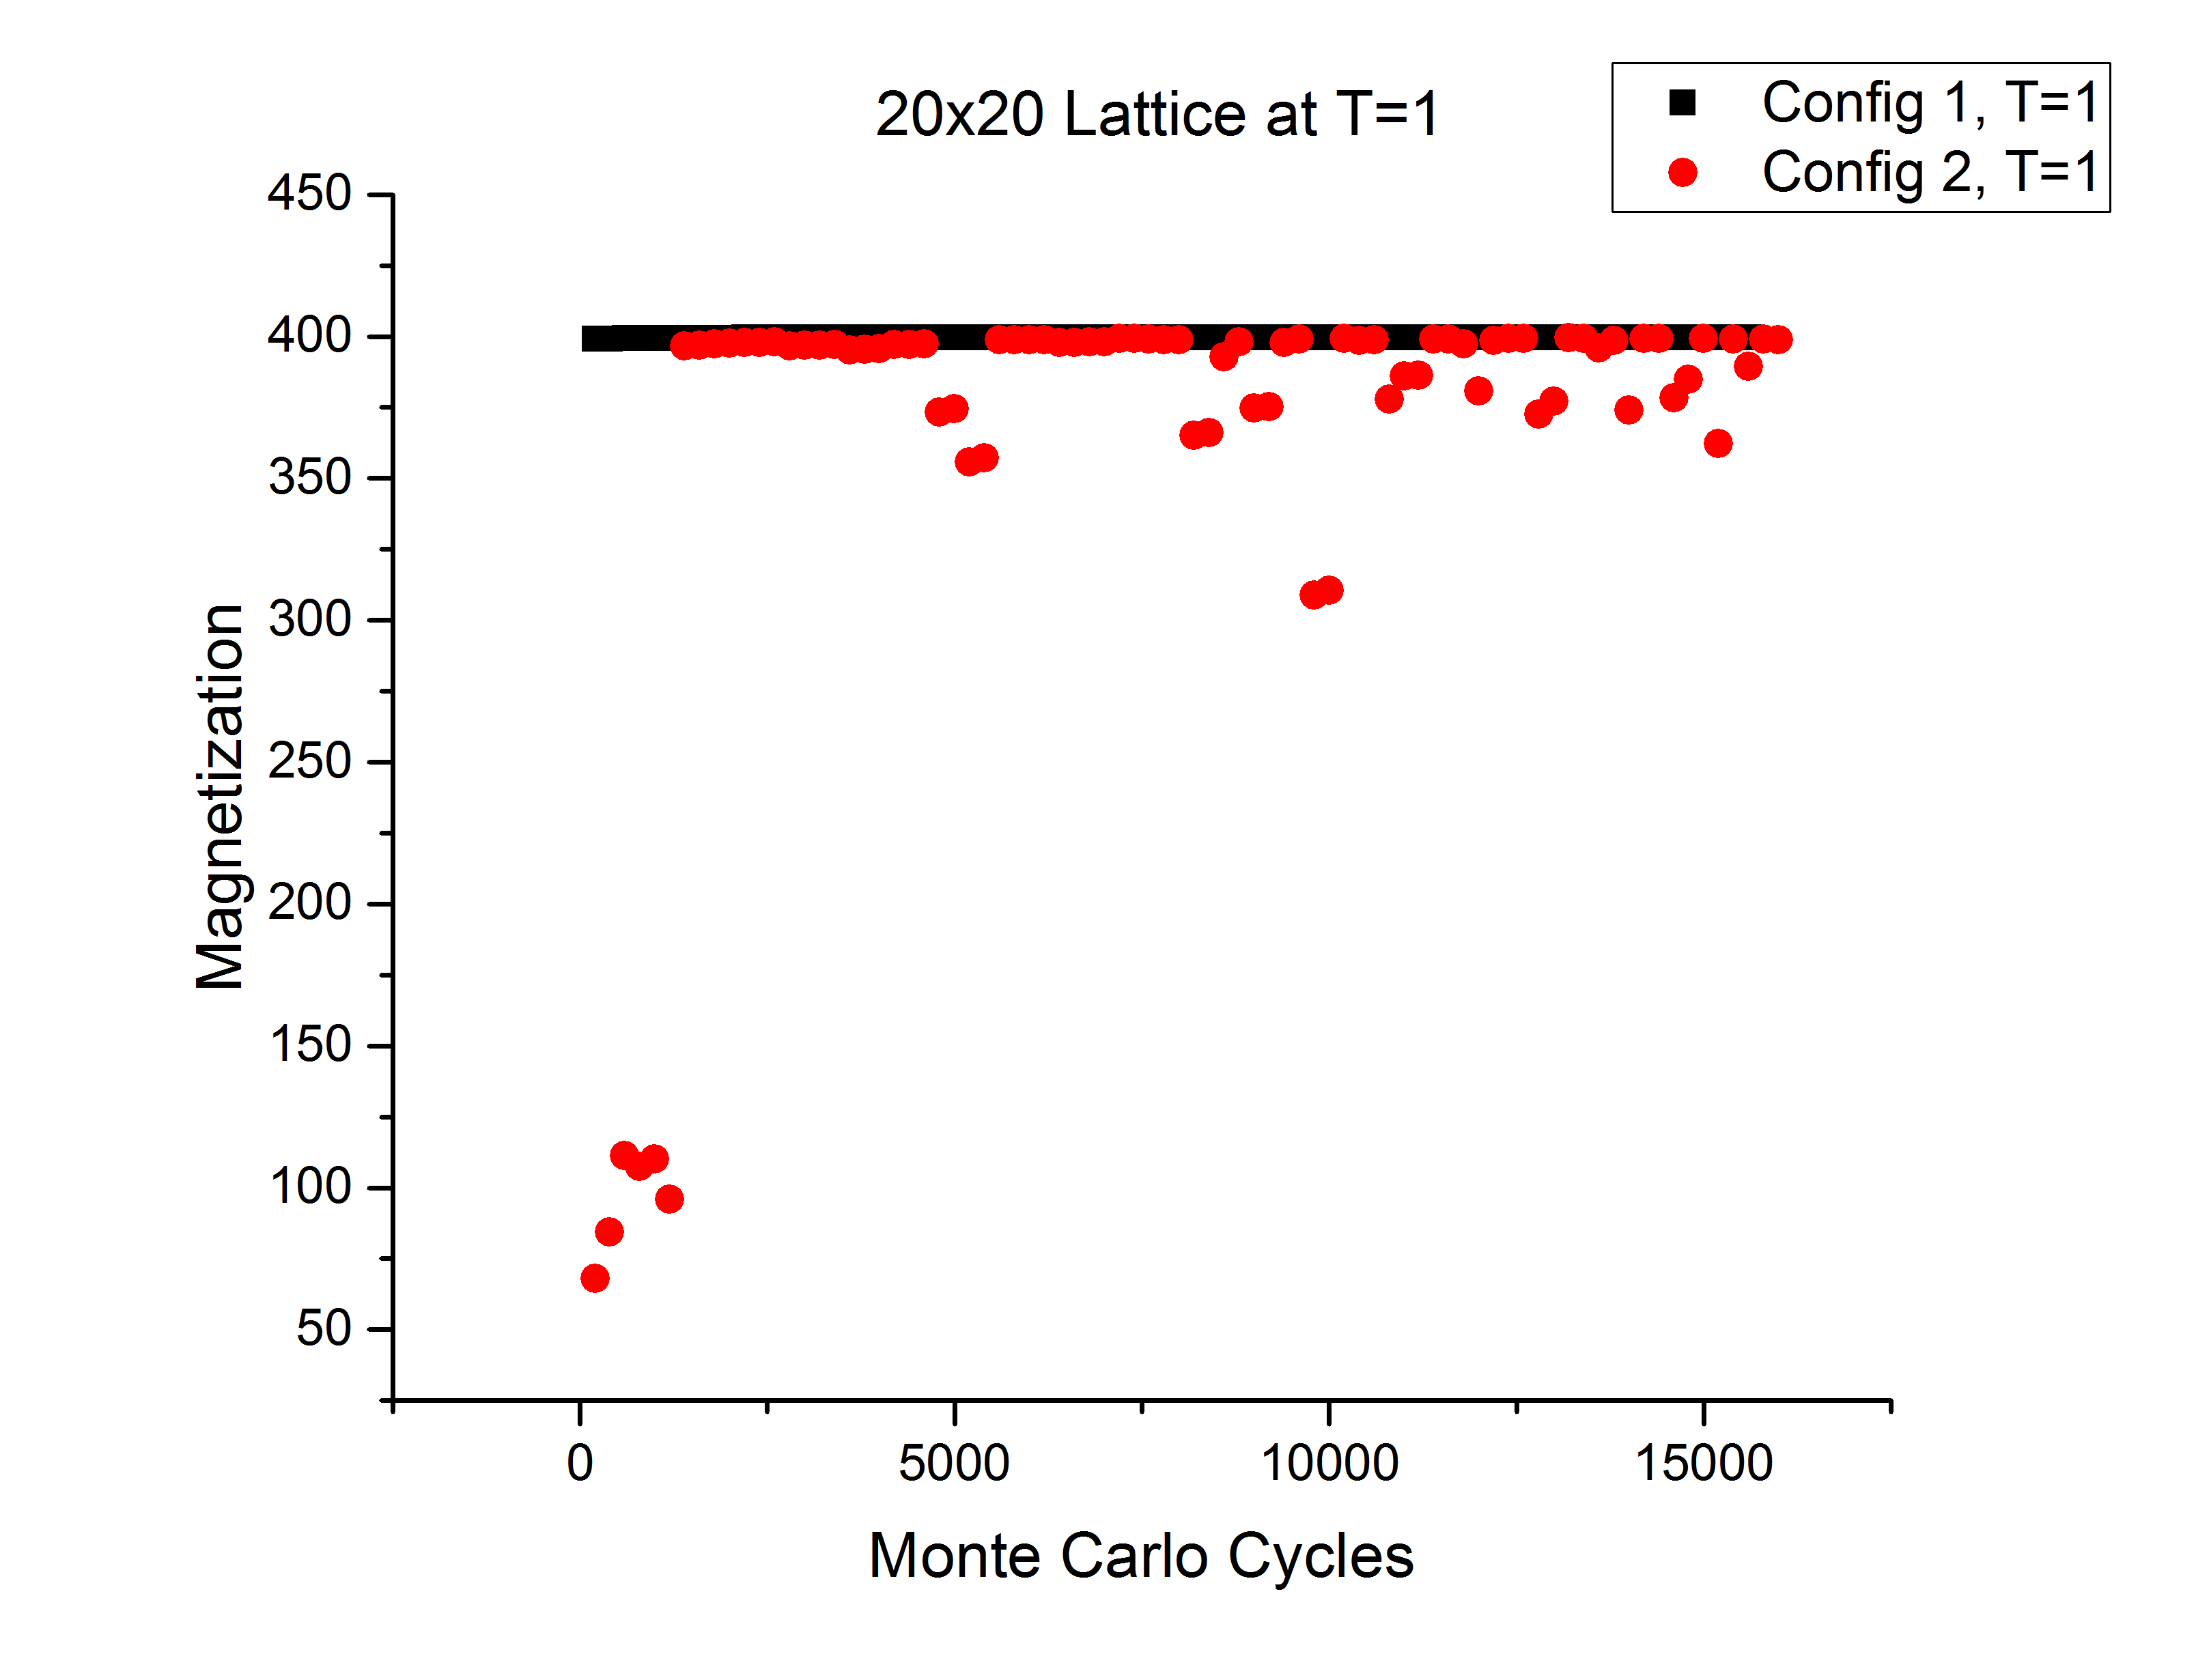
\includegraphics[width=3in]{Graph03.png}
			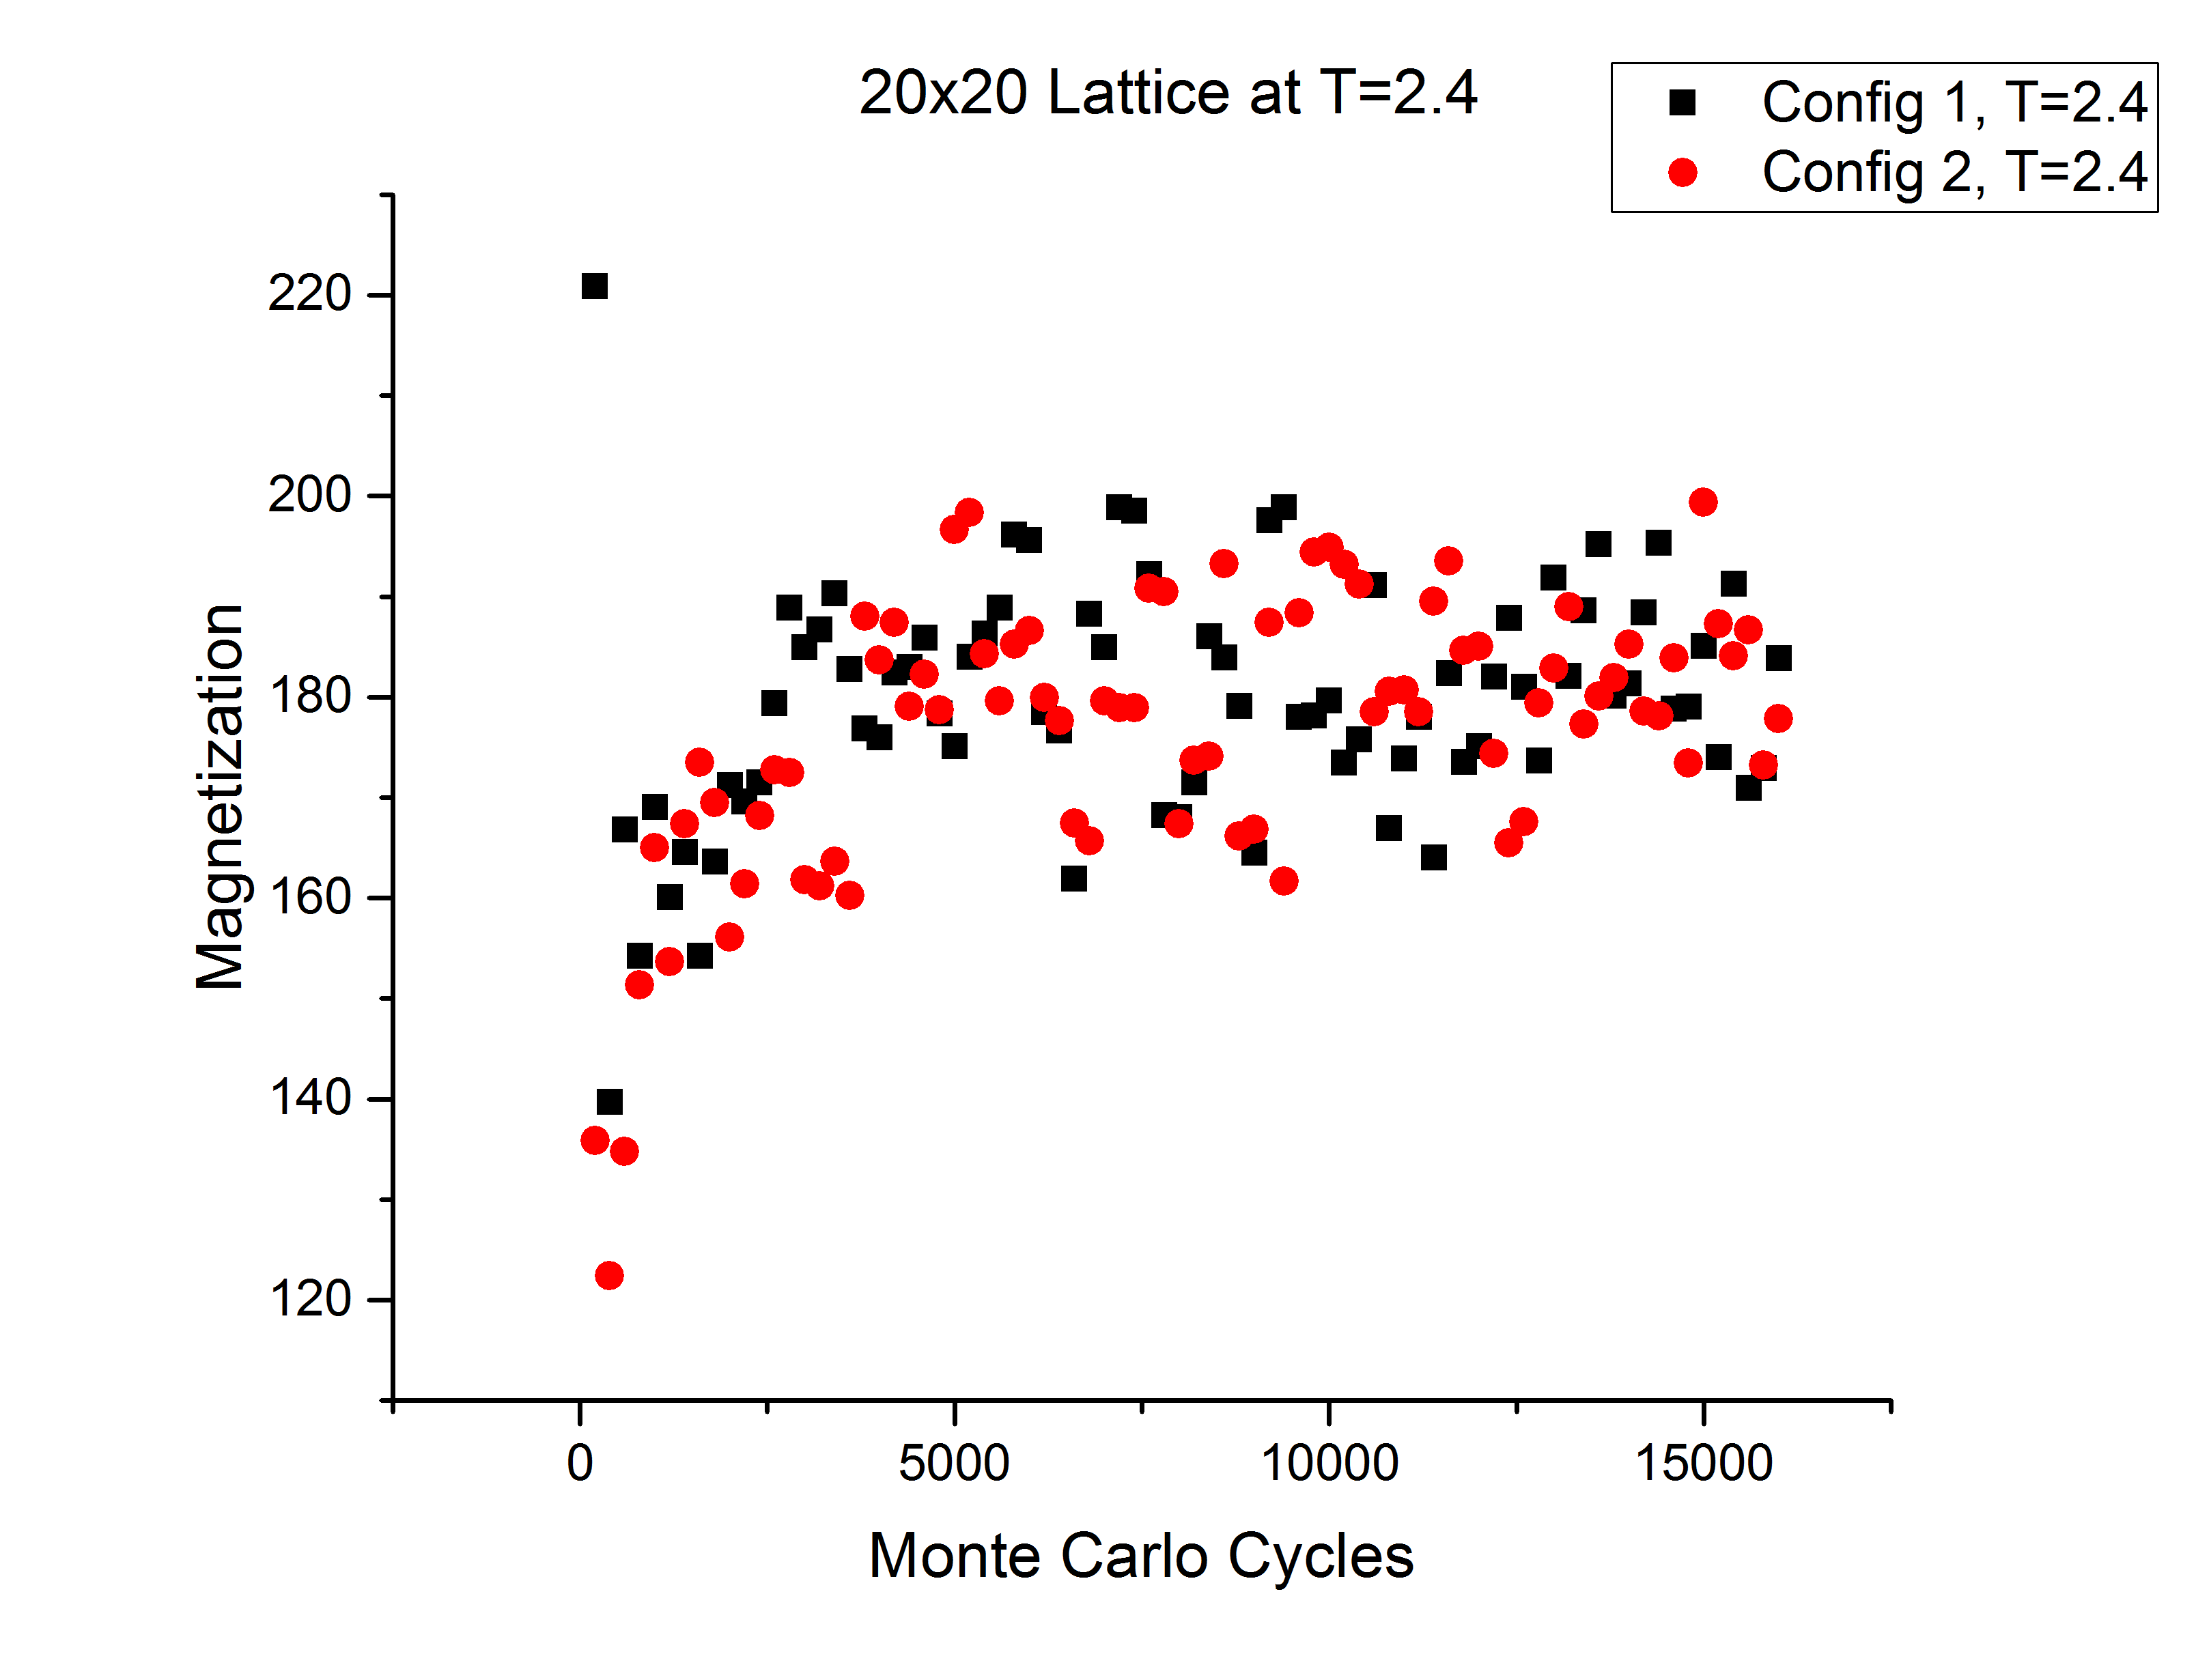
\includegraphics[width=3in]{Graph04.png}
			
			
			\caption{\label{Magnetization} Average Magnetization for different temperatures and initial configurations (Left) T=1 (Right) T=2.4}
		\end{figure}
	Fig. ~\ref{Accptance} shows how the number of accepted configurations change as the number of Monte Carlo cycles are changed. Everything in red is for when the system is at T=1, while everything in black is for when the system is at T=2.4. The main thing to point out in this figure is that when at T=1 there are very few changes in the configuration that are accepted and the value increases linearly very slowly. For the random starting configuration there are quite a few jumps in the number of configuration flips, while for the starting all aligned starting configuration there are no jumps what so ever. The more interesting case is for when T=2.4. In this case it appears as though the starting configuration doesn't matter at all. Like the case for T=1 the number of configurations increase linearly with the number of Monte Carlo cycles, except now the number of configuration flips are several orders of magnitude larger than in the previous case.
		\begin{figure}
			
			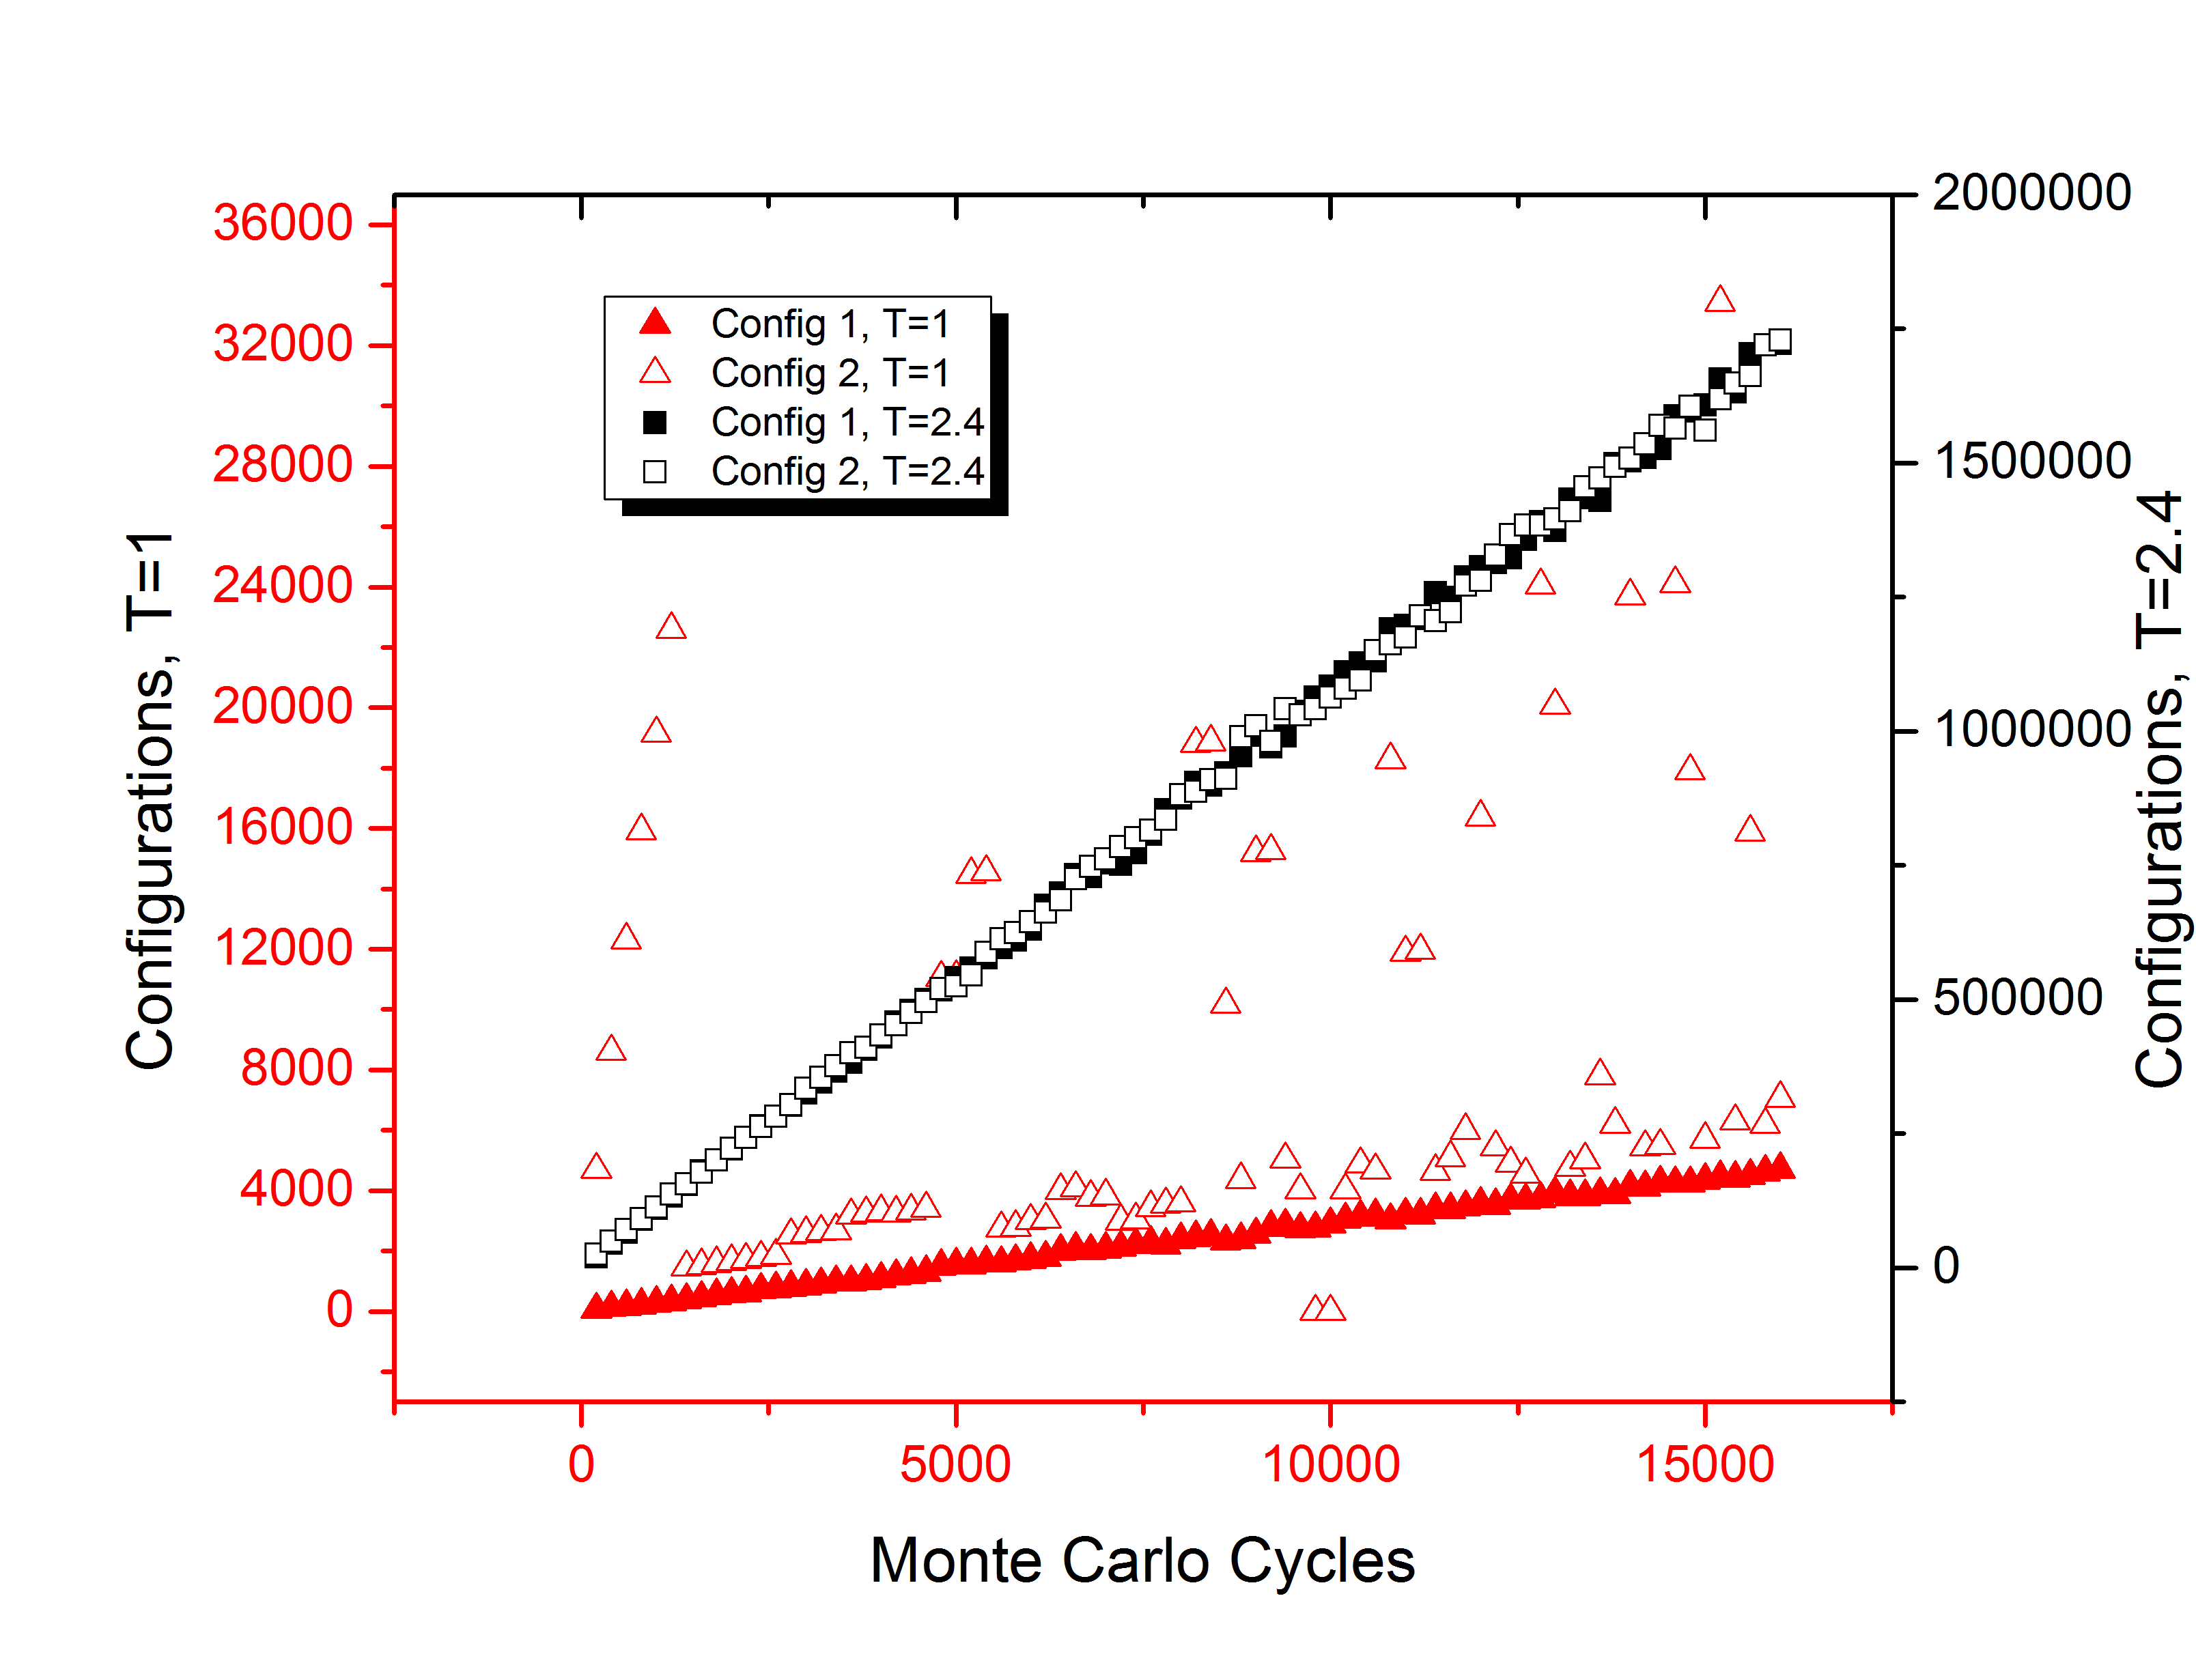
\includegraphics[width=4in]{Graph05.png}
			
			
			
			\caption{\label{Accptance} Number of configurations accepted as a function of Monte Carlo Cycles for T=1 and T=2.4 and for the two above mentioned starting configurations}
		\end{figure}
	The final thing that was looked at for the 20x20 matrix was the probability distribution of the energy for different starting configurations and temperatures. These distributions were calculated once the system reached equilibrium. The distributions in Fig. ~\ref{Probability} shows that for both configurations with T=1 the probability distribution is very small, placing the data into a histogram would show a single large spike. This is what is seen in Fig. ~\ref{Energy}, where after equilibrium is reached there is no variance in the energy at all. For T=2.4 Fig.~\ref{Probability} shows a distribution with quite a bit of spread, this is also supported by what is seen in Fig.~\ref{Energy}.
	
		
		
		
		
		
		
		
		
			\begin{figure}
				
				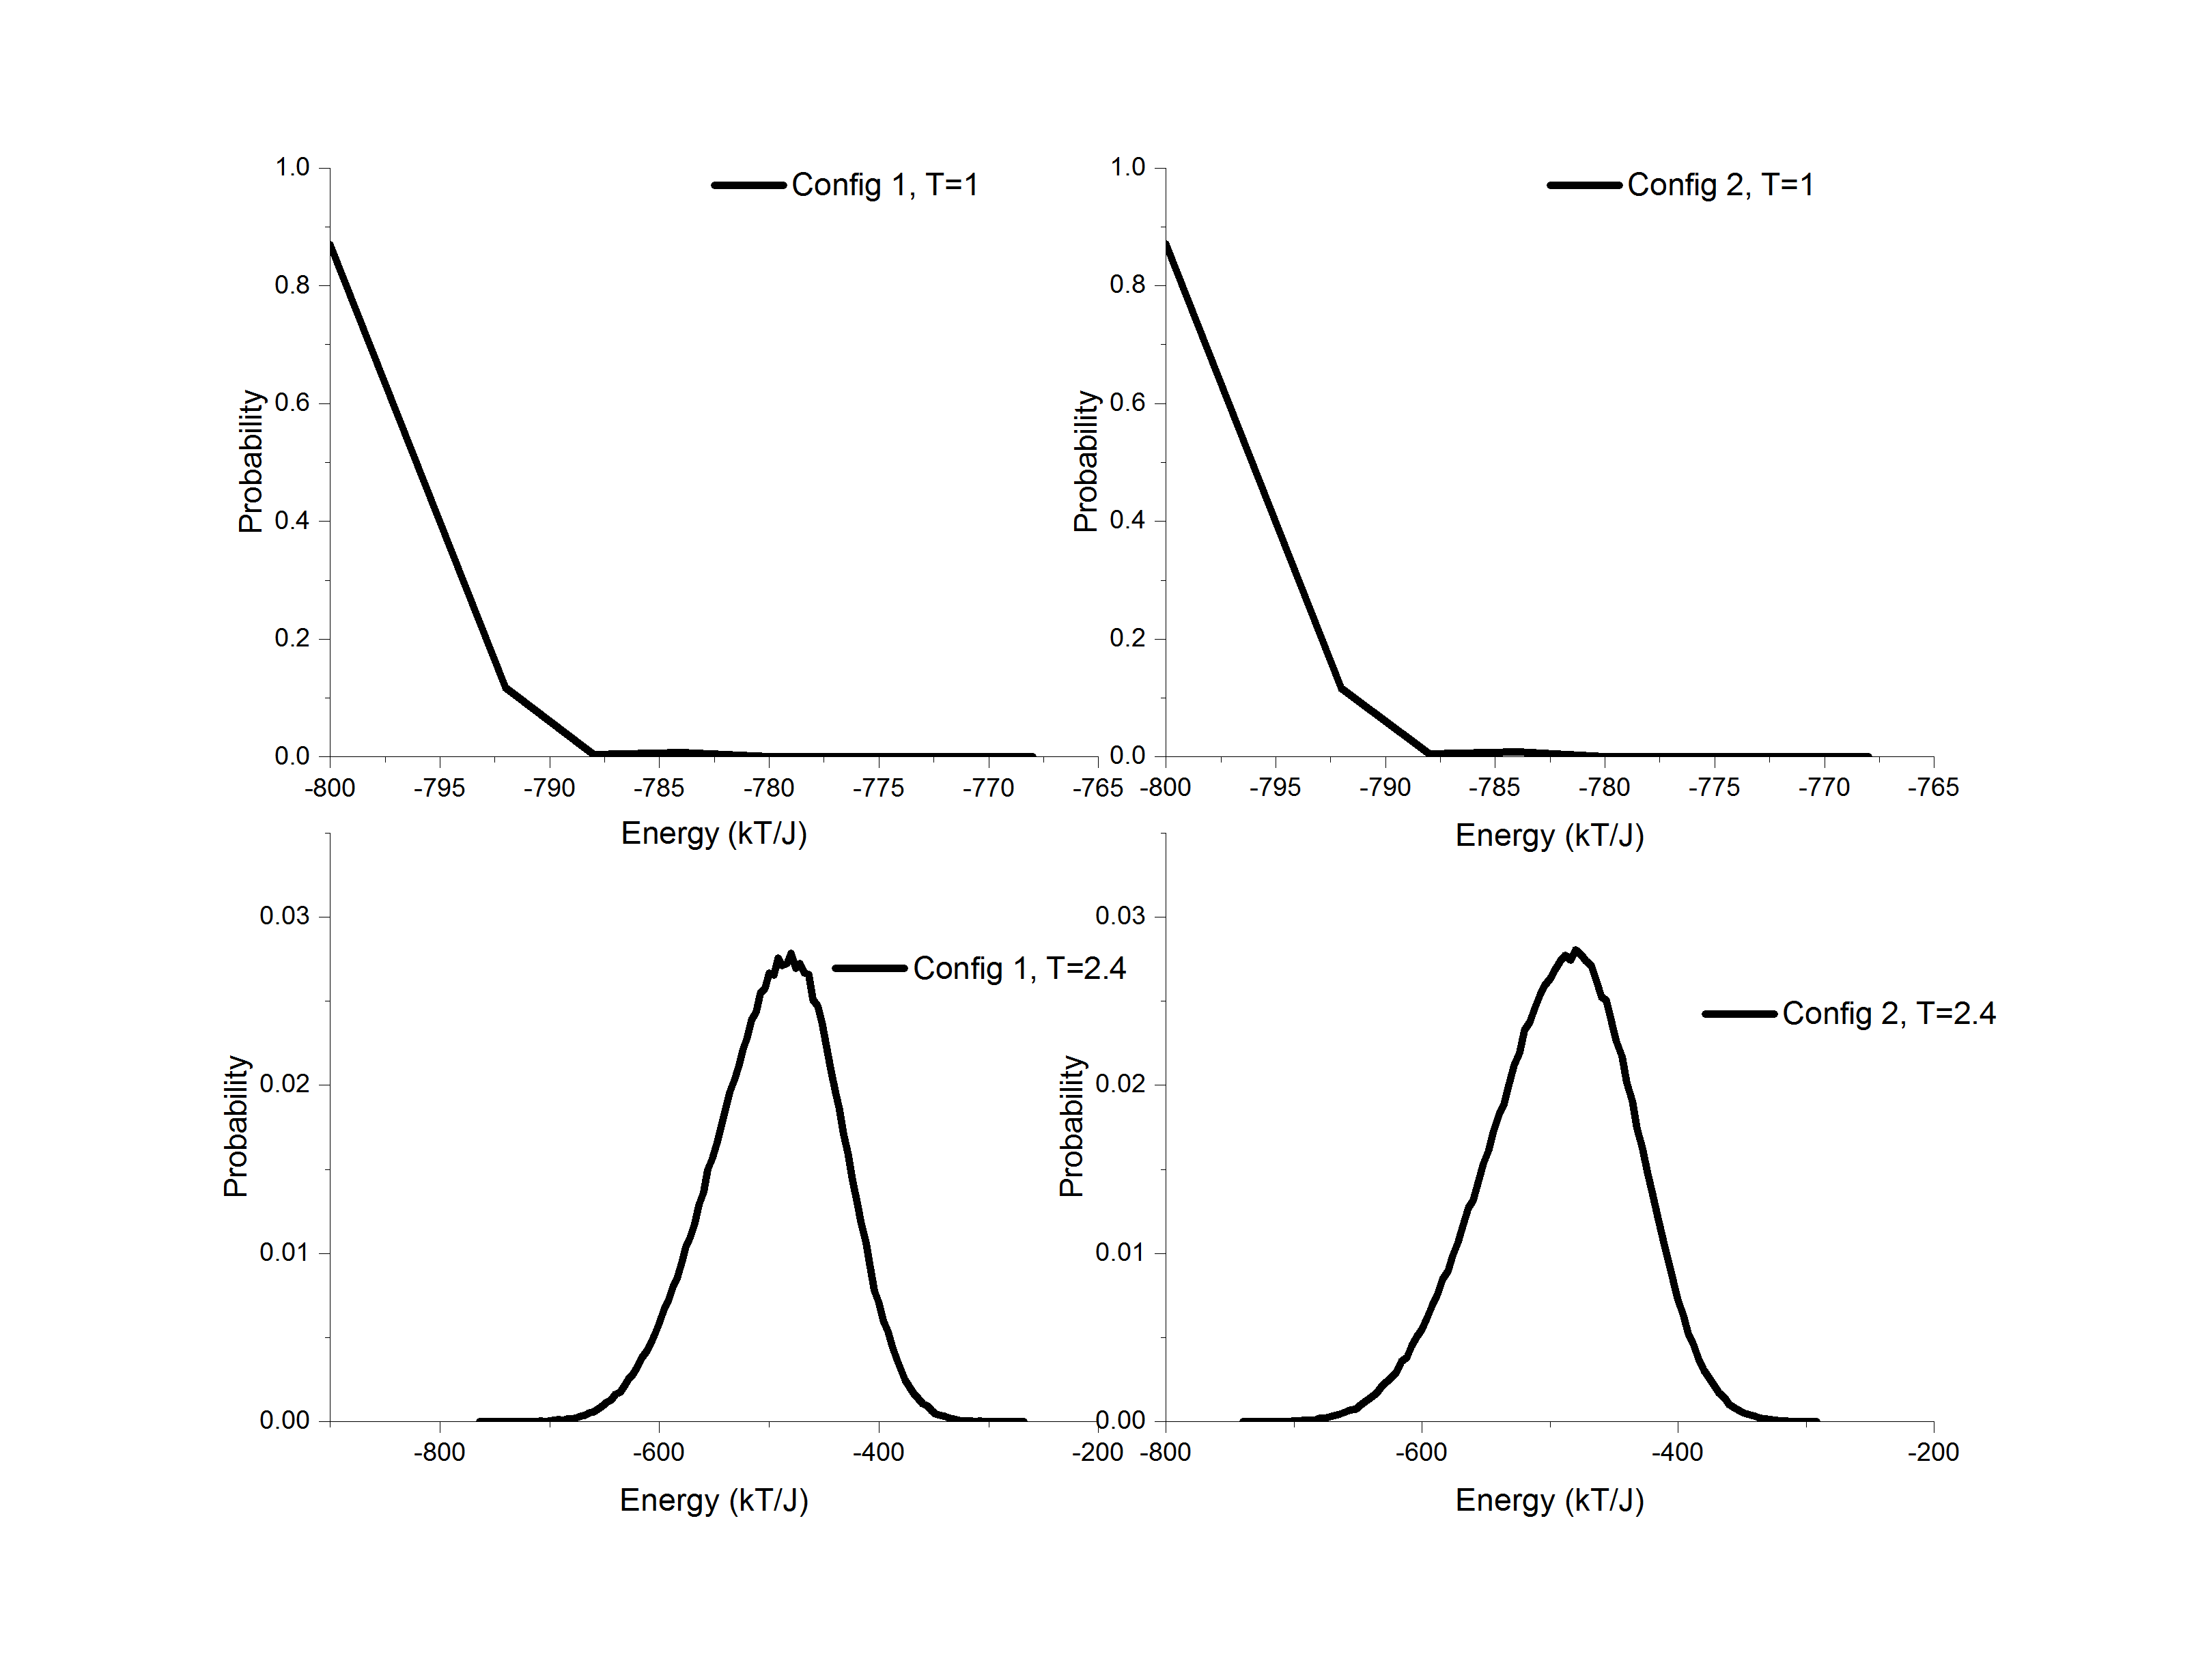
\includegraphics[width=6in]{Graph06.png}
				
				
				
				\caption{\label{Probability} Probability distribution of the energy}
			\end{figure}
		
		
\subsection{Temperature Dependence of the Ising Model}		
		
		The final thing that was investigated was how the Ising Model behaves for different lattice sizes over a range of temperatures and then try and extract a value for the critical temperature. The lattice sizes that were used were 20x20, 40x40, 60x60 and 80x80. These runs were done using 500,000 Monte-Carlo cycles with a temperature step size of 0.05 so as to be able to see the phase transition. Fig.~\ref{Thermo} shows  the graphs for average energy, magnetization, specific heat and susceptibility per particle for the above mentioned lattice sizes. For all of the quantities investigated the values below and above the critical temperature are the same across all lattice size except for the magnetization. However, in the range of the critical temperature all of the values are drastically different except for in the energy, but even there they are fairly close. In the magnetization it is very clear that as the size of the lattice increases the behavior of a jump discontinuity becomes more and more apparent, where below the critical temperature all spins are correlated and above they are randomly distributed. Looking at the figures for both specific heat and susceptibility it is clear that there is a phase transition taking place characterized by the lambda shape the graphs take. It is clear that as the size of the lattice increases we can clearly see that the critical temperature decreases, approaching the value of 2.26 calculated by Osanger.
		
		The next step is to now find what the critical temperature is by using the calculated values for the critical temperature and $T_c(L)-T_c(\infty)=aL^{-1}$. To do this however the code was ran again over a temperature scale around the critical temperatures for all of the lattice sizes using a step length of just 0.01 and doing 1,000,000 Monte Carlo cycles. Once the calculations were rerun the critical temperatures were extracted from both the specific heat and the susceptibility by simply looking at the graphs and finding where it looked like they diverged. Once the critical temperatures were obtained the next step is to actually find the critical temperature as the lattice goes to infinity using the above equation. Now, this equation has two unknown variables a and $T_c(\infty)$, so we basically have 4 equations with 2 unknowns for both the specific heat and susceptibility critical temperatures that were derived. So what I did to account for this was knowing that a and $T_c(\infty)$ should be the same for all lattice sizes I solved the equation using the critical temperatures for susceptibility 6 times in an odometric fashion. Once these values were obtained I simply took the average over all 6 critical temperatures and a values. These values are shown in tables 4 and 5, as well as there averages and standard deviations. Looking at averages the average for the susceptibility is closer to that of the critical temperature calculated by Onsanger of 2.269 than that calculated from the temperatures of the specific heats. This would make sense though because it was more difficult to actually see a sharp peak in the values of the specific heat as the temperature goes through the critical point. However, if only using the standard deviation as our error bars then we are well within the range of Onsangers value for both of our values of the critical temperature.
		
		
			\begin{table}
				\begin{center}
					\caption{Critical Temperatures for Different Lattice Sizes}
					\begin{tabular}{c c c}
						\hline\hline
						Lattice Size & $T_c$ from Specific Heat & $T_c$ from Susceptibility  \\ 
						\hline
						20x20 & 2.32 & 2.37\\
						40x40 & 2.29 & 2.31 \\
						60x60 & 2.28 & 2.3 \\
						80x80 & 2.27 & 2.9  \\
					
						
						\hline
					\end{tabular}
				\end{center}
			\end{table}
		
		
		\begin{table}
			\begin{center}
				\caption{Values for a and $T_c(\infty)$ using Specific Heat Temps}
				\begin{tabular}{c c c}
					\hline\hline
					Lattice Size & a & $T_c$  \\ 
					\hline
					20x20/40x40 & 1.2 & 2.26\\
					20x20/60x60 & 1.2 & 2.26 \\
					20x20/80x80 & 1.333 & 2.25333 \\
					40x40/60x60 & 1.2 & 2.26  \\
					40x40/80x80 &   1.6 & 2.25    \\
					60x60/80x80 &  2.4  &  2.24  \\
					Average & 1.4888 & 2.2538 \\
					Standard Deviation & 0.431 & 0.0213 \\
					\hline
				\end{tabular}
			\end{center}
		\end{table}
			\begin{table}
				\begin{center}
					\caption{Values for a and $T_c(\infty)$ using Susceptibility Temps}
					\begin{tabular}{c c c}
						\hline\hline
						Lattice Size & a & $T_c$  \\ 
						\hline
						20x20/40x40 & 2.4 & 2.25\\
						20x20/60x60 & 2.1 & 2.265 \\
						20x20/80x80 & 2.1333 & 2.26333 \\
						40x40/60x60 & 1.2 & 2.28  \\
						40x40/80x80 &   1.6 & 2.27    \\
						60x60/80x80 &  2.4  &  2.26  \\
						Average & 1.9722 & 2.2647 \\
						Standard Deviation & 0.436 & 0.0134 \\
						\hline
					\end{tabular}
				\end{center}
			\end{table}
			\begin{figure}
				
				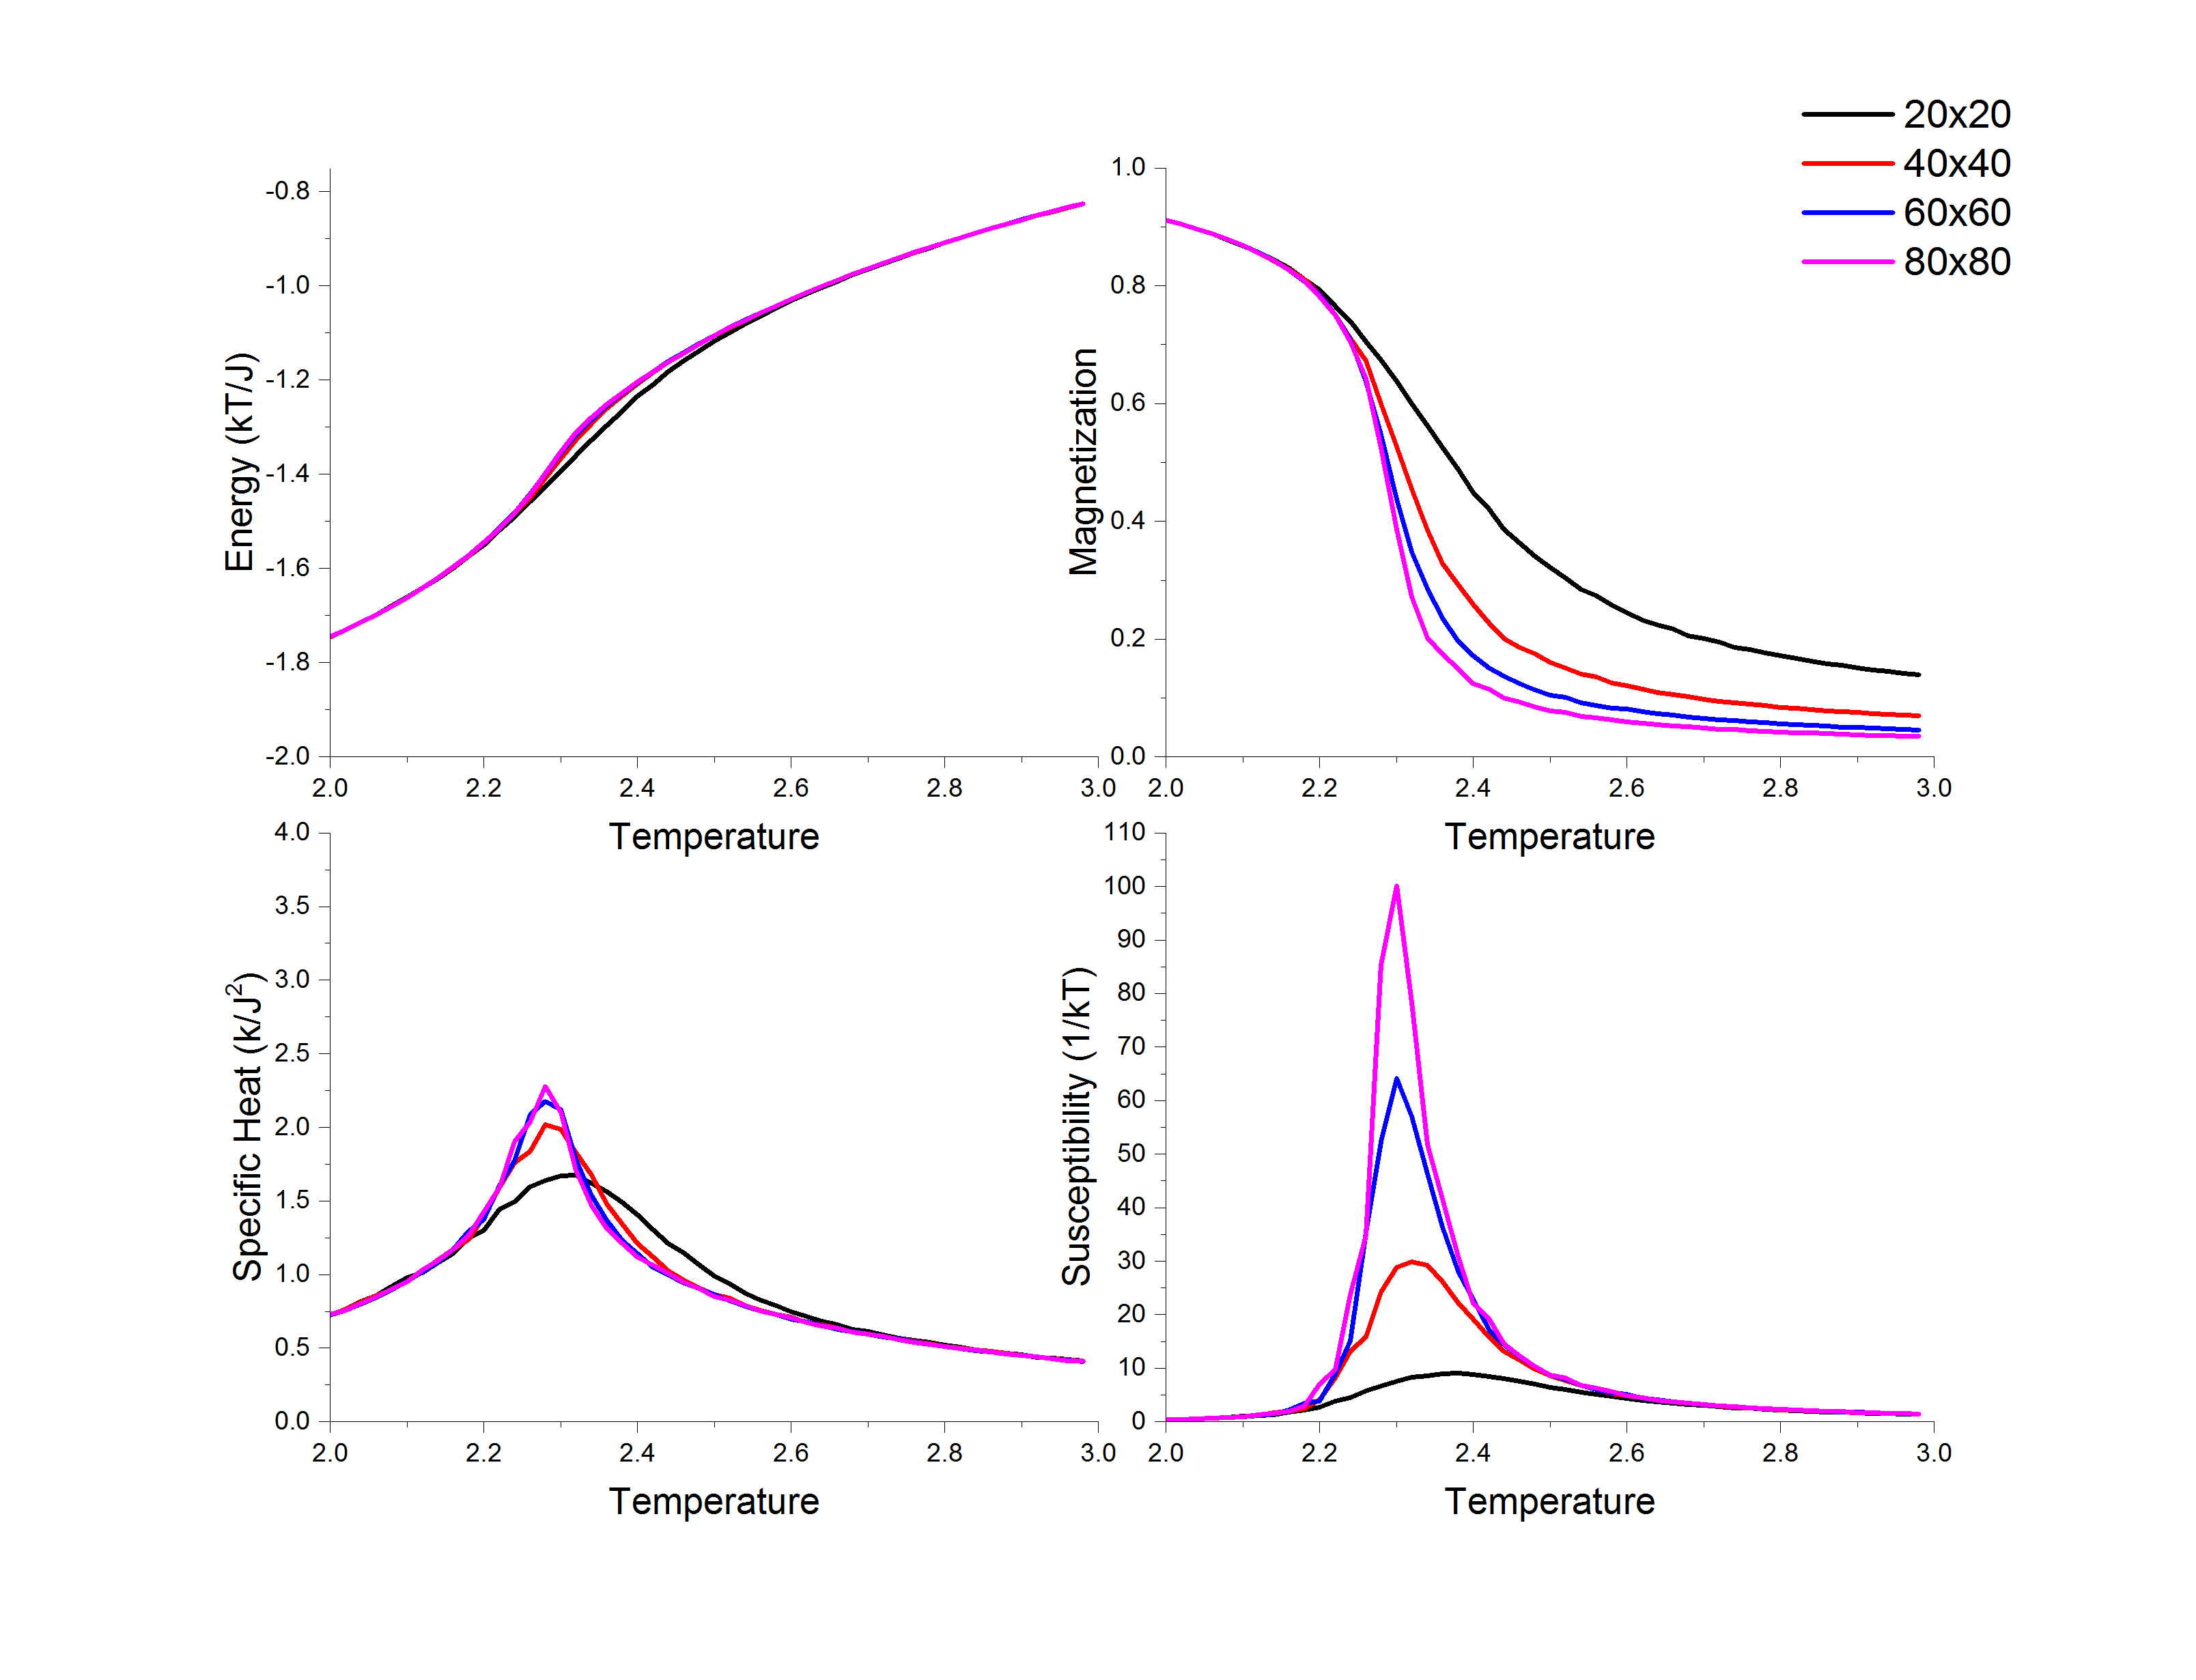
\includegraphics[width=6in]{Awesomegraph.png}
				
				
				
				\caption{\label{Thermo} Thermodynamic quantities for different lattice sizes }
			\end{figure}
		
		
		
		
		
\section{Conclusion}
In this study we were able to accurately predict the value of the critical temperature within error bars that Onsanger's analytical result provides using the Ising model in its simplest form. Along with this it was found that to ensure a fast convergence of the Ising model to equilibrium it is important to choose a starting particle configuration that is representative of the starting temperature. Also, below the critical point fluctuations in the values of the thermodynamic quantities are very small, meaning that meaningful results can be obtained with very few Monte Carlo cycles. However, once past the critical point there are a large number of fluctuations around a mean, meaning that in order to get results that mean anything a large number of Monte Carlo cycles are needed to gather enough statistics. Also, for this case before data can be taken a number of Monte Carlo cycles have to be run though to reach the equilibrium.

 
\begin{thebibliography}{9}
	\bibitem{1}
	M. H, Jensen, Project 4 Introduction
	
	\bibitem{2}
	M. H, Jensen, Phys 904 Lecture Notes
	
	\bibitem{3}
	Wikipedia, Ernst Ising, 2016, https://en.wikipedia.org/wiki/Ernst Ising 
	
	\bibitem{4} 
	Statistical Mechanics Notes On the Ising Model for Zelevinski Recitation session
	
	\bibitem{5}
	Wikipedia, Ising Model, 2016, https://en.wikipedia.org/wiki/Ising Model
	
\end{thebibliography}






\end{document}	